% Created by tikzDevice version 0.6.2-92-0ad2792 on 2013-02-07 01:46:30
% !TEX encoding = UTF-8 Unicode
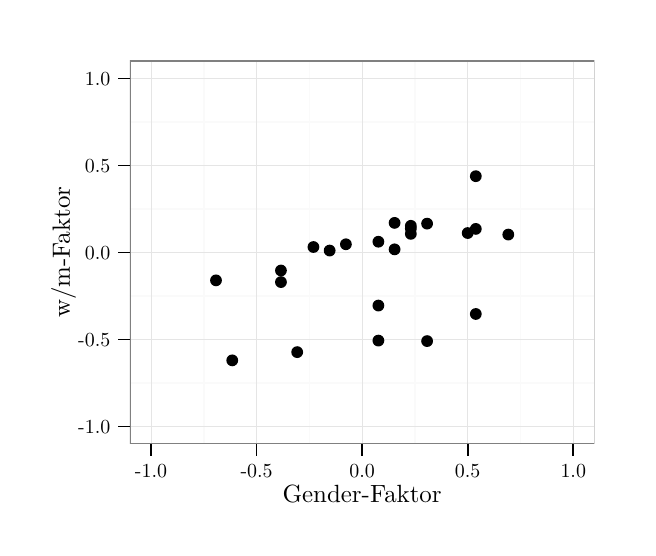
\begin{tikzpicture}[x=1pt,y=1pt]
\definecolor[named]{fillColor}{rgb}{1.00,1.00,1.00}
\path[use as bounding box,fill=fillColor,fill opacity=0.00] (0,0) rectangle (216.81,180.67);
\begin{scope}
\path[clip] (  0.00,  0.00) rectangle (216.81,180.67);
\definecolor[named]{drawColor}{rgb}{1.00,1.00,1.00}
\definecolor[named]{fillColor}{rgb}{1.00,1.00,1.00}

\path[draw=drawColor,line width= 0.6pt,line join=round,line cap=round,fill=fillColor] (  0.00,  0.00) rectangle (216.81,180.67);
\end{scope}
\begin{scope}
\path[clip] ( 36.95, 30.32) rectangle (204.76,168.63);
\definecolor[named]{fillColor}{rgb}{1.00,1.00,1.00}

\path[fill=fillColor] ( 36.95, 30.32) rectangle (204.76,168.63);
\definecolor[named]{drawColor}{rgb}{0.98,0.98,0.98}

\path[draw=drawColor,line width= 0.6pt,line join=round] ( 36.95, 52.32) --
	(204.76, 52.32);

\path[draw=drawColor,line width= 0.6pt,line join=round] ( 36.95, 83.76) --
	(204.76, 83.76);

\path[draw=drawColor,line width= 0.6pt,line join=round] ( 36.95,115.19) --
	(204.76,115.19);

\path[draw=drawColor,line width= 0.6pt,line join=round] ( 36.95,146.63) --
	(204.76,146.63);

\path[draw=drawColor,line width= 0.6pt,line join=round] ( 63.65, 30.32) --
	( 63.65,168.63);

\path[draw=drawColor,line width= 0.6pt,line join=round] (101.79, 30.32) --
	(101.79,168.63);

\path[draw=drawColor,line width= 0.6pt,line join=round] (139.93, 30.32) --
	(139.93,168.63);

\path[draw=drawColor,line width= 0.6pt,line join=round] (178.07, 30.32) --
	(178.07,168.63);
\definecolor[named]{drawColor}{rgb}{0.90,0.90,0.90}

\path[draw=drawColor,line width= 0.2pt,line join=round] ( 36.95, 36.60) --
	(204.76, 36.60);

\path[draw=drawColor,line width= 0.2pt,line join=round] ( 36.95, 68.04) --
	(204.76, 68.04);

\path[draw=drawColor,line width= 0.2pt,line join=round] ( 36.95, 99.47) --
	(204.76, 99.47);

\path[draw=drawColor,line width= 0.2pt,line join=round] ( 36.95,130.91) --
	(204.76,130.91);

\path[draw=drawColor,line width= 0.2pt,line join=round] ( 36.95,162.34) --
	(204.76,162.34);

\path[draw=drawColor,line width= 0.2pt,line join=round] ( 44.58, 30.32) --
	( 44.58,168.63);

\path[draw=drawColor,line width= 0.2pt,line join=round] ( 82.72, 30.32) --
	( 82.72,168.63);

\path[draw=drawColor,line width= 0.2pt,line join=round] (120.86, 30.32) --
	(120.86,168.63);

\path[draw=drawColor,line width= 0.2pt,line join=round] (159.00, 30.32) --
	(159.00,168.63);

\path[draw=drawColor,line width= 0.2pt,line join=round] (197.14, 30.32) --
	(197.14,168.63);
\definecolor[named]{fillColor}{rgb}{0.00,0.00,0.00}

\path[fill=fillColor] (109.12,100.13) circle (  2.13);

\path[fill=fillColor] (114.99,102.40) circle (  2.13);

\path[fill=fillColor] (126.73,103.32) circle (  2.13);

\path[fill=fillColor] (126.73, 67.60) circle (  2.13);

\path[fill=fillColor] (138.46,106.16) circle (  2.13);

\path[fill=fillColor] (161.93, 77.21) circle (  2.13);

\path[fill=fillColor] ( 73.92, 60.45) circle (  2.13);

\path[fill=fillColor] ( 91.52, 88.74) circle (  2.13);

\path[fill=fillColor] ( 91.52, 92.92) circle (  2.13);

\path[fill=fillColor] (173.67,105.91) circle (  2.13);

\path[fill=fillColor] ( 68.05, 89.36) circle (  2.13);

\path[fill=fillColor] ( 97.39, 63.43) circle (  2.13);

\path[fill=fillColor] (103.26,101.41) circle (  2.13);

\path[fill=fillColor] (126.73, 80.26) circle (  2.13);

\path[fill=fillColor] (132.59,100.56) circle (  2.13);

\path[fill=fillColor] (132.59,110.13) circle (  2.13);

\path[fill=fillColor] (161.93,127.00) circle (  2.13);

\path[fill=fillColor] (144.33,109.86) circle (  2.13);

\path[fill=fillColor] (138.46,108.05) circle (  2.13);

\path[fill=fillColor] (138.46,109.07) circle (  2.13);

\path[fill=fillColor] (144.33, 67.42) circle (  2.13);

\path[fill=fillColor] (159.00,106.46) circle (  2.13);

\path[fill=fillColor] (161.93,107.95) circle (  2.13);
\definecolor[named]{drawColor}{rgb}{0.50,0.50,0.50}

\path[draw=drawColor,line width= 0.6pt,line join=round,line cap=round] ( 36.95, 30.32) rectangle (204.76,168.63);
\end{scope}
\begin{scope}
\path[clip] (  0.00,  0.00) rectangle (216.81,180.67);
\definecolor[named]{drawColor}{rgb}{0.00,0.00,0.00}

\node[text=drawColor,anchor=base east,inner sep=0pt, outer sep=0pt, scale=  0.72] at ( 29.84, 34.12) {-1.0};

\node[text=drawColor,anchor=base east,inner sep=0pt, outer sep=0pt, scale=  0.72] at ( 29.84, 65.56) {-0.5};

\node[text=drawColor,anchor=base east,inner sep=0pt, outer sep=0pt, scale=  0.72] at ( 29.84, 96.99) {0.0};

\node[text=drawColor,anchor=base east,inner sep=0pt, outer sep=0pt, scale=  0.72] at ( 29.84,128.43) {0.5};

\node[text=drawColor,anchor=base east,inner sep=0pt, outer sep=0pt, scale=  0.72] at ( 29.84,159.86) {1.0};
\end{scope}
\begin{scope}
\path[clip] (  0.00,  0.00) rectangle (216.81,180.67);
\definecolor[named]{drawColor}{rgb}{0.00,0.00,0.00}

\path[draw=drawColor,line width= 0.6pt,line join=round] ( 32.69, 36.60) --
	( 36.95, 36.60);

\path[draw=drawColor,line width= 0.6pt,line join=round] ( 32.69, 68.04) --
	( 36.95, 68.04);

\path[draw=drawColor,line width= 0.6pt,line join=round] ( 32.69, 99.47) --
	( 36.95, 99.47);

\path[draw=drawColor,line width= 0.6pt,line join=round] ( 32.69,130.91) --
	( 36.95,130.91);

\path[draw=drawColor,line width= 0.6pt,line join=round] ( 32.69,162.34) --
	( 36.95,162.34);
\end{scope}
\begin{scope}
\path[clip] (  0.00,  0.00) rectangle (216.81,180.67);
\definecolor[named]{drawColor}{rgb}{0.00,0.00,0.00}

\path[draw=drawColor,line width= 0.6pt,line join=round] ( 44.58, 26.05) --
	( 44.58, 30.32);

\path[draw=drawColor,line width= 0.6pt,line join=round] ( 82.72, 26.05) --
	( 82.72, 30.32);

\path[draw=drawColor,line width= 0.6pt,line join=round] (120.86, 26.05) --
	(120.86, 30.32);

\path[draw=drawColor,line width= 0.6pt,line join=round] (159.00, 26.05) --
	(159.00, 30.32);

\path[draw=drawColor,line width= 0.6pt,line join=round] (197.14, 26.05) --
	(197.14, 30.32);
\end{scope}
\begin{scope}
\path[clip] (  0.00,  0.00) rectangle (216.81,180.67);
\definecolor[named]{drawColor}{rgb}{0.00,0.00,0.00}

\node[text=drawColor,anchor=base,inner sep=0pt, outer sep=0pt, scale=  0.72] at ( 44.58, 18.24) {-1.0};

\node[text=drawColor,anchor=base,inner sep=0pt, outer sep=0pt, scale=  0.72] at ( 82.72, 18.24) {-0.5};

\node[text=drawColor,anchor=base,inner sep=0pt, outer sep=0pt, scale=  0.72] at (120.86, 18.24) {0.0};

\node[text=drawColor,anchor=base,inner sep=0pt, outer sep=0pt, scale=  0.72] at (159.00, 18.24) {0.5};

\node[text=drawColor,anchor=base,inner sep=0pt, outer sep=0pt, scale=  0.72] at (197.14, 18.24) {1.0};
\end{scope}
\begin{scope}
\path[clip] (  0.00,  0.00) rectangle (216.81,180.67);
\definecolor[named]{drawColor}{rgb}{0.00,0.00,0.00}

\node[text=drawColor,anchor=base,inner sep=0pt, outer sep=0pt, scale=  0.90] at (120.86,  9.03) {Gender-Faktor};
\end{scope}
\begin{scope}
\path[clip] (  0.00,  0.00) rectangle (216.81,180.67);
\definecolor[named]{drawColor}{rgb}{0.00,0.00,0.00}

\node[text=drawColor,rotate= 90.00,anchor=base,inner sep=0pt, outer sep=0pt, scale=  0.90] at ( 15.23, 99.47) {w/m-Faktor};
\end{scope}
\end{tikzpicture}
